\documentclass[12pt]{beamer}
%\documentclass[12pt]{article}
%\usepackage[noxcolor]{beamerarticle}

\usepackage{pgfpages}
\usepackage{handoutWithNotes}


\setbeameroption{show notes on second screen=right}

\setbeamertemplate{note page}{\pagecolor{white!5}\insertnote}\usepackage{palatino}

\begin{document}

\begin{frame}
  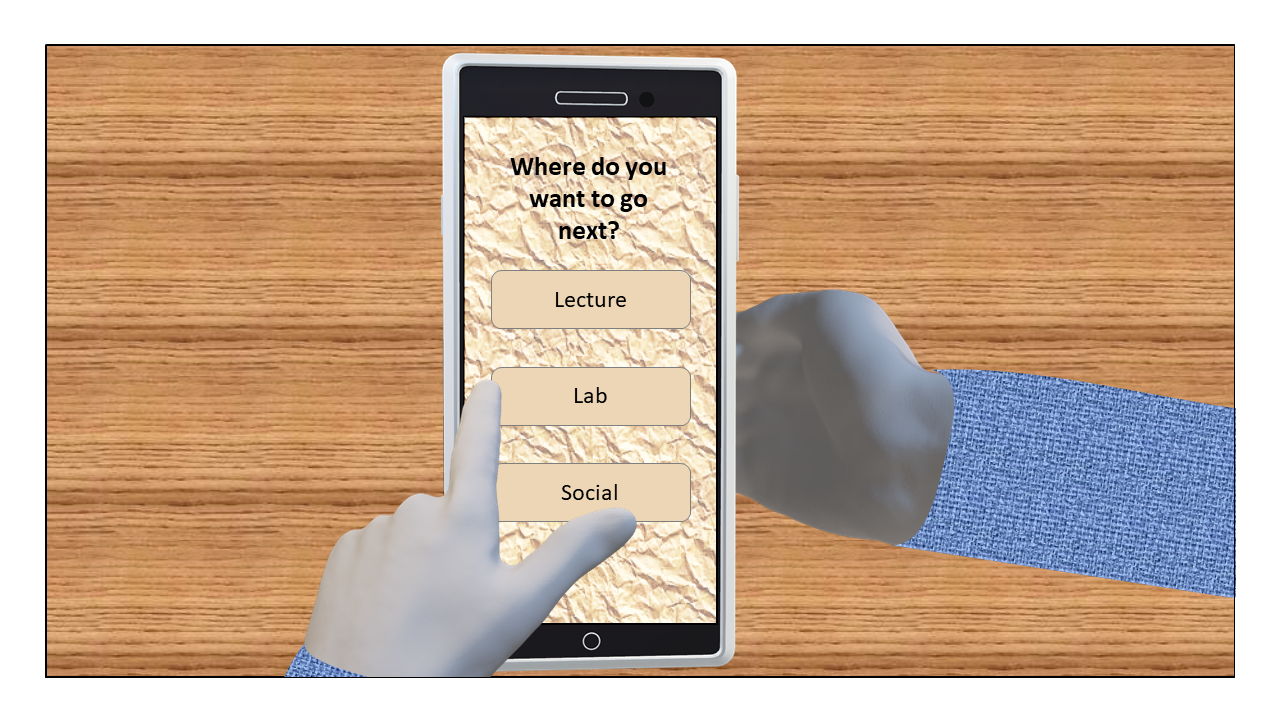
\includegraphics[width=\paperwidth]{./figures/initial_storyboards/Slide2.png}
  \note{
    Alan can choose what kind of location he wants to go next.
    He sees three buttons on the middle of the screen, and he taps one.    
  }
\end{frame}

\begin{frame}
  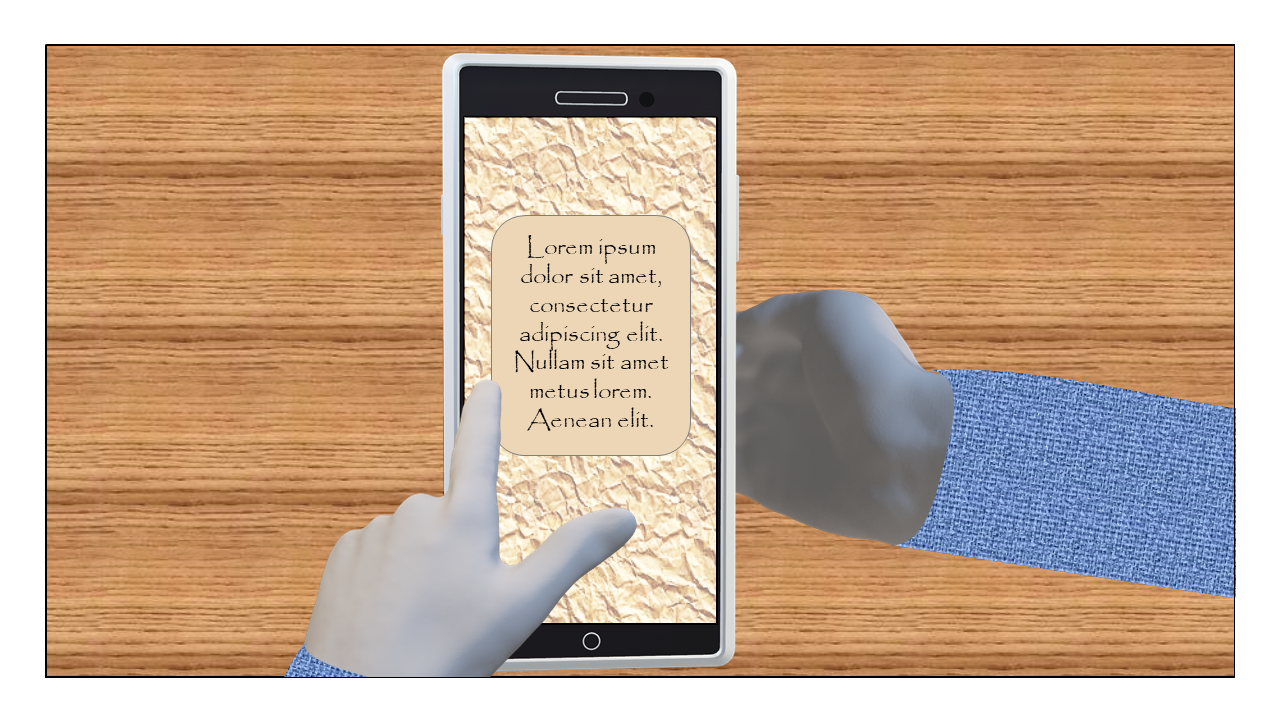
\includegraphics[width=\paperwidth]{./figures/initial_storyboards/Slide3.png}
  \note{
    The screen changes – the buttons are hidden, and are replaced by a singular riddle.
    He takes some time to think about where the riddle may lead him, what location it can describe.
    Once he is confident in his solution, he locks his phone, puts it in his pocket, and heads to the location.    
  }
\end{frame}

\begin{frame}
  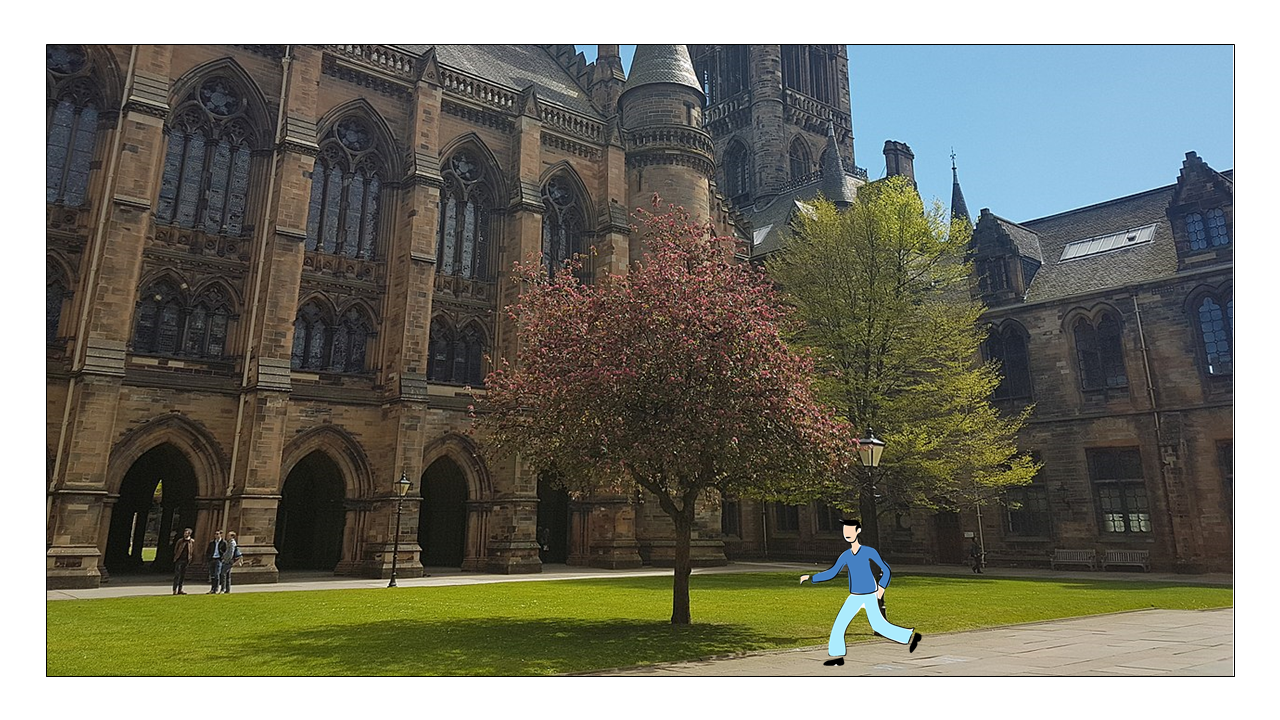
\includegraphics[width=\paperwidth]{./figures/initial_storyboards/Slide4.png}
  \note{
    Alan heads to the building he believes the solution is in.
    He has his phone in his pocket, as he does not need it for navigation.
    The app does not show him where the solution of the riddle is or how to get there.
    When he is uncertain about his solution, he steps to the side to not block anyone’s path, and looks at the riddle again to refresh his memory.    
  }
\end{frame}

\begin{frame}
  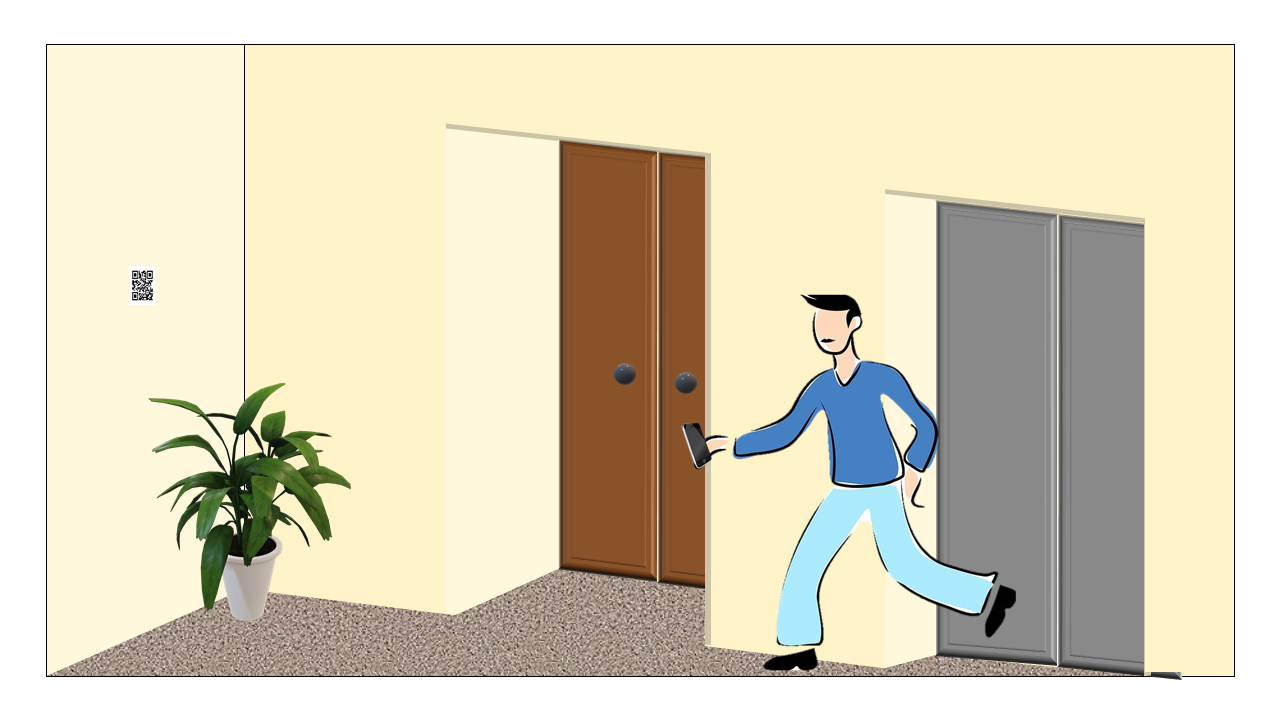
\includegraphics[width=\paperwidth]{./figures/initial_storyboards/Slide5.png}
  \note{
    Alan steps out of the elevator and notices the QR code.
    He is happy that his intuition was correct, and he solved the riddle correctly.
    He proceeds to the code, not blocking other people’s entrance to the lab.
    He takes out his phone from his pocket to open the app and check in at the checkpoint.    
  }
\end{frame}

\begin{frame}
  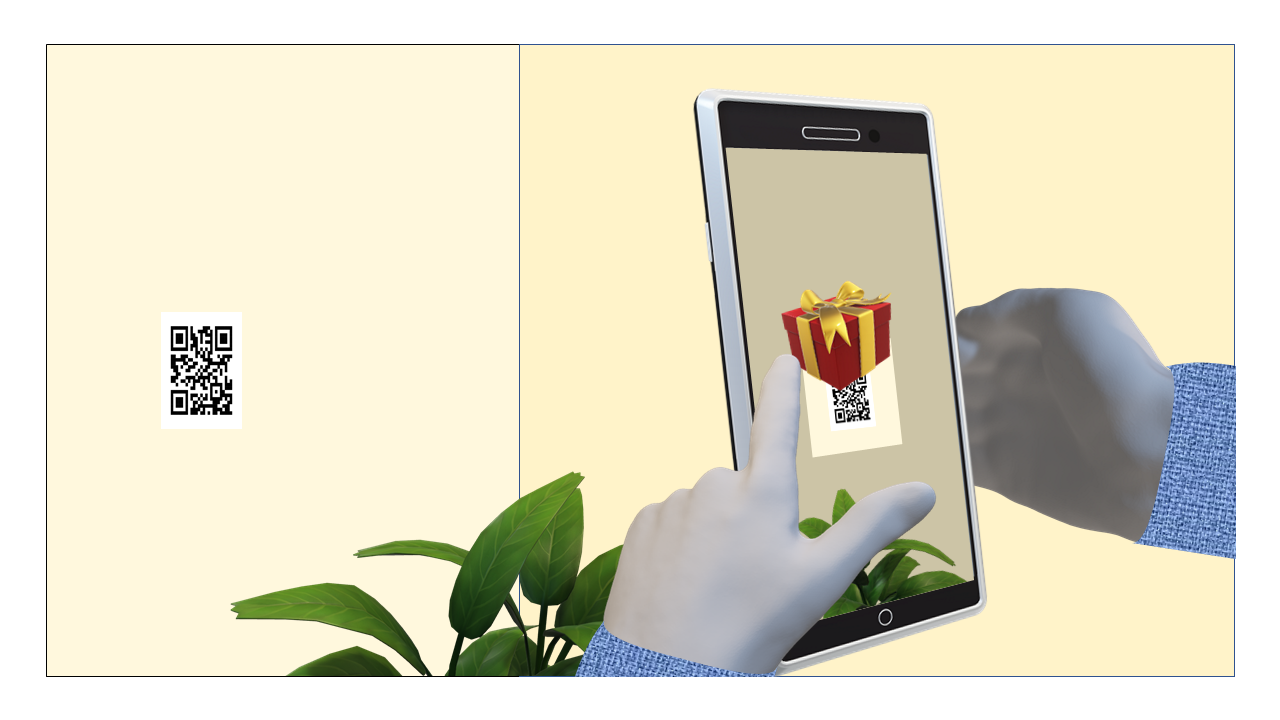
\includegraphics[width=\paperwidth]{./figures/initial_storyboards/Slide6.png}
  \note{
    Alan taps on the camera button at bottom of the screen.
    The screen quickly changes as the build in camera feature opens in the app.
    The screen shows a bounding box with grey tint on the screen outside the bounding box – this shows Alan that he needs to move the QR code inside the bounding box to scan it.
    The AR representation of a checkpoint item then appears on the screen on top of the QR code, and moves in space with the phone as long as the QR code stays within bounding box.    
  }
\end{frame}

\begin{frame}
  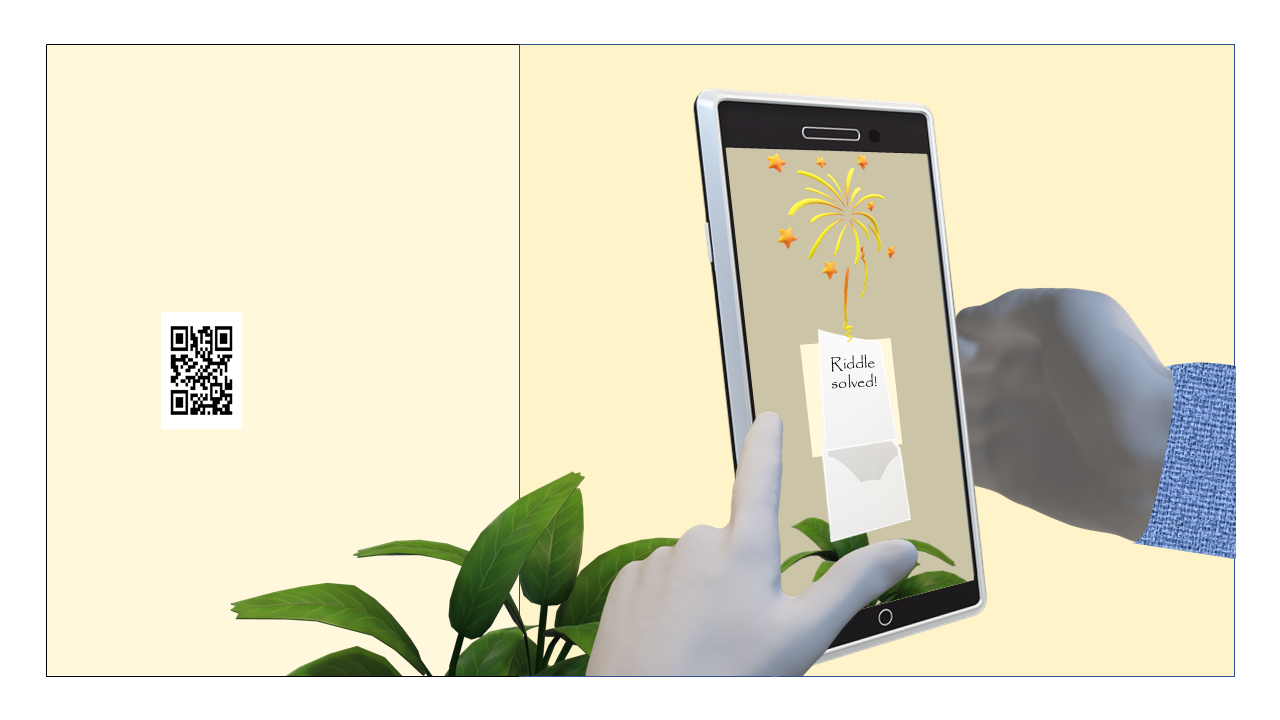
\includegraphics[width=\paperwidth]{./figures/initial_storyboards/Slide7.png}
  \note{
    Alan taps on the checkpoint item he is presented with.
    If the riddle was solved correctly and Alan arrived at the location the riddle told him to, the phone vibrates three times to signal to him he succeeded. At the same time, a small, triumphant sound effect plays to collaborate the physical feedback.
    The screen also changes, and a small animation of an envelope opening happens.
    From the envelope fireworks appear and a popup tells Alan he scanned the location and the riddle was solved.
    The app then tells him all the XP he’s gained, if he has levelled up, and if he gained any new freebies.    
  }
\end{frame}

\begin{frame}
  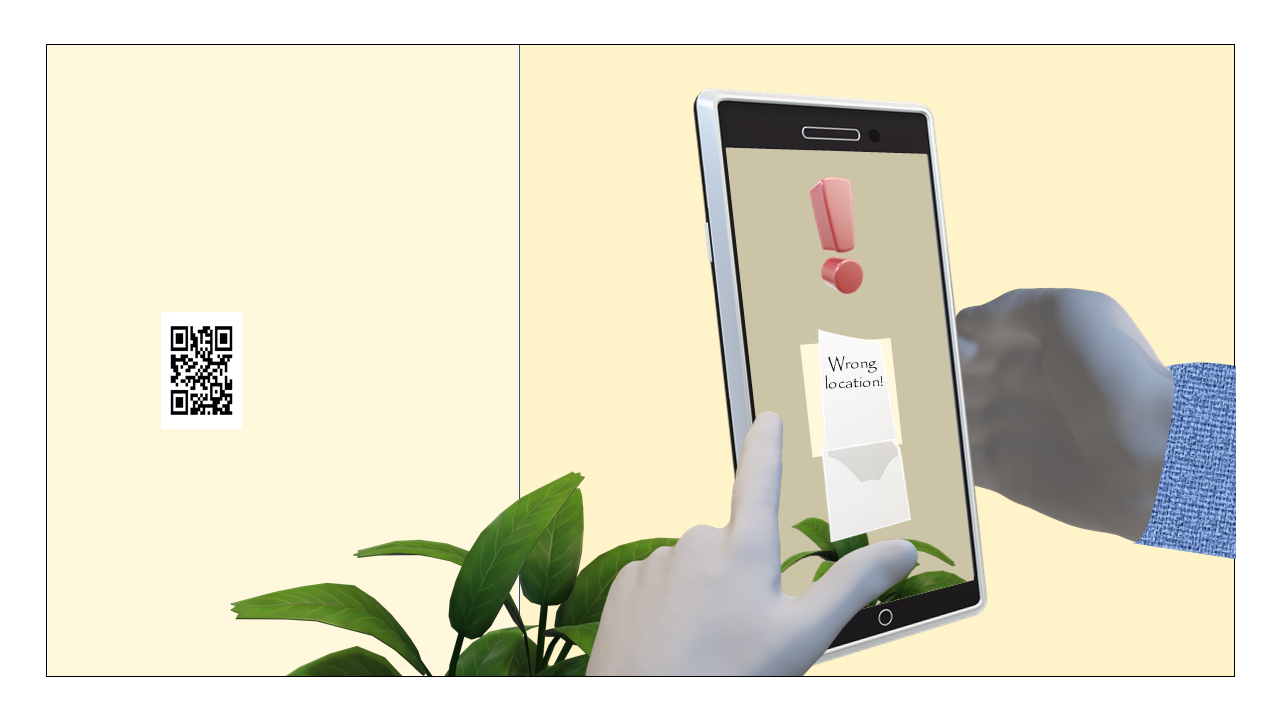
\includegraphics[width=\paperwidth]{./figures/initial_storyboards/Slide8.png}
  \note{
    Alan taps on the checkpoint item he is presented with.
    If the riddle was solved incorrectly and Alan arrived at a location different to what the riddle told him to, the phone vibrates twice to signal to him he got the answer wrong.
    The screen also changes, and a small animation of an envelope opening happens.
    From the envelope a red exclamation point appears and a popup tells Alan that he is in the wrong location.
    The application then presents him with the option to register this location as the wrong answer to the riddle, or to not register the check-in and allow him to try figure out the correct answer.    
  }
\end{frame}

\begin{frame}
    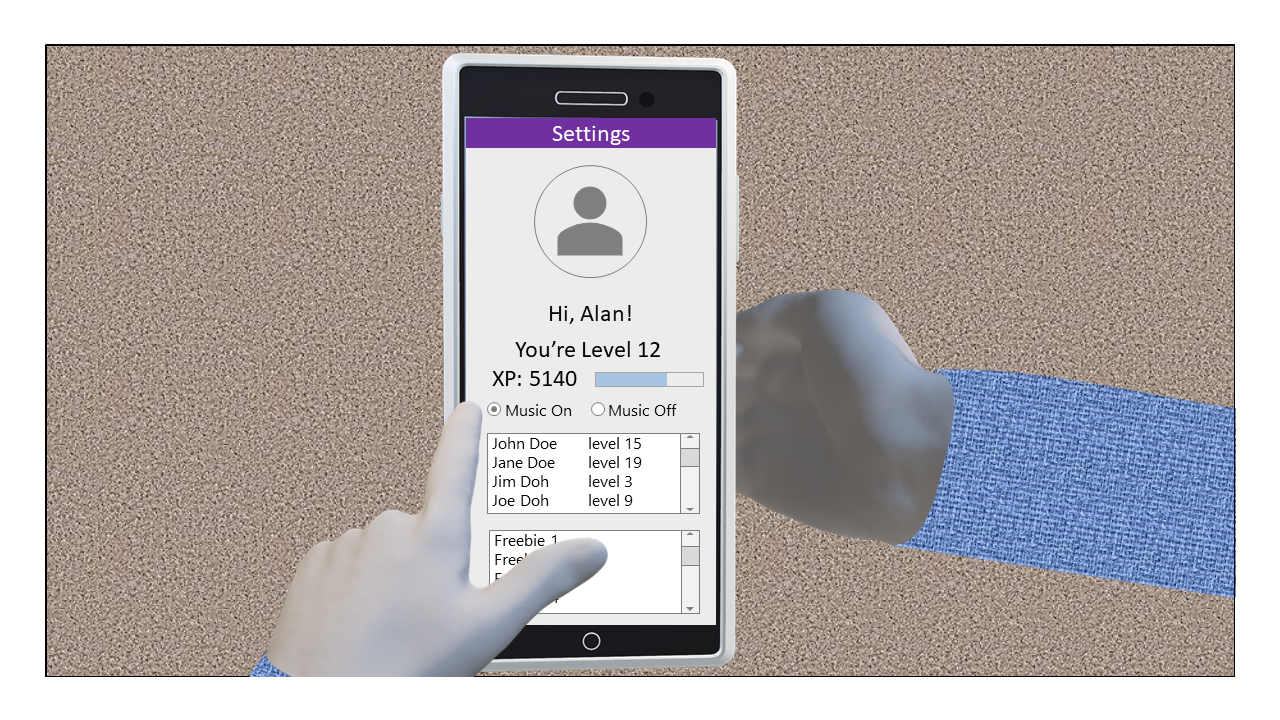
\includegraphics[width=\paperwidth]{./figures/initial_storyboards/Slide9.png}
    \note{
        After having completed a checkpoint, Alan views his in-game progress.
He does so by tapping on the Settings button at the main screen. 
He views his XP, his list of friends, his in-game level, his badges earned, and can also adjust the app settings or log out if he wants to.
He is pleased to see he is close to levelling up, and with the new level, he is to gain new freebies.
    }
  \end{frame}
  
\end{document}